\subsection{Galaxy Clustering}\label{sec:lia}

%\subsubsection{Motivation}

\subsubsection{The Effect}
The simplest statistic that
characterizes the angular distribution of galaxies on the sky is the
angular correlation function, $w(\vec\theta_1,\vec\theta_2)$, which
quantifies the excess probability over random that a galaxy will be
found at $\vec\theta_2$ given that there is a galaxy at
$\vec\theta_1$. In the isotropic case, the angular correlation function depends only on the angular distance
between the two positions: $w=w(\vert\vec\theta_1-\vec\theta_2\vert)$. The \atf\ effect here means
that $w$ depends also on the location on the sky.

\begin{figure}
  \begin{center}
    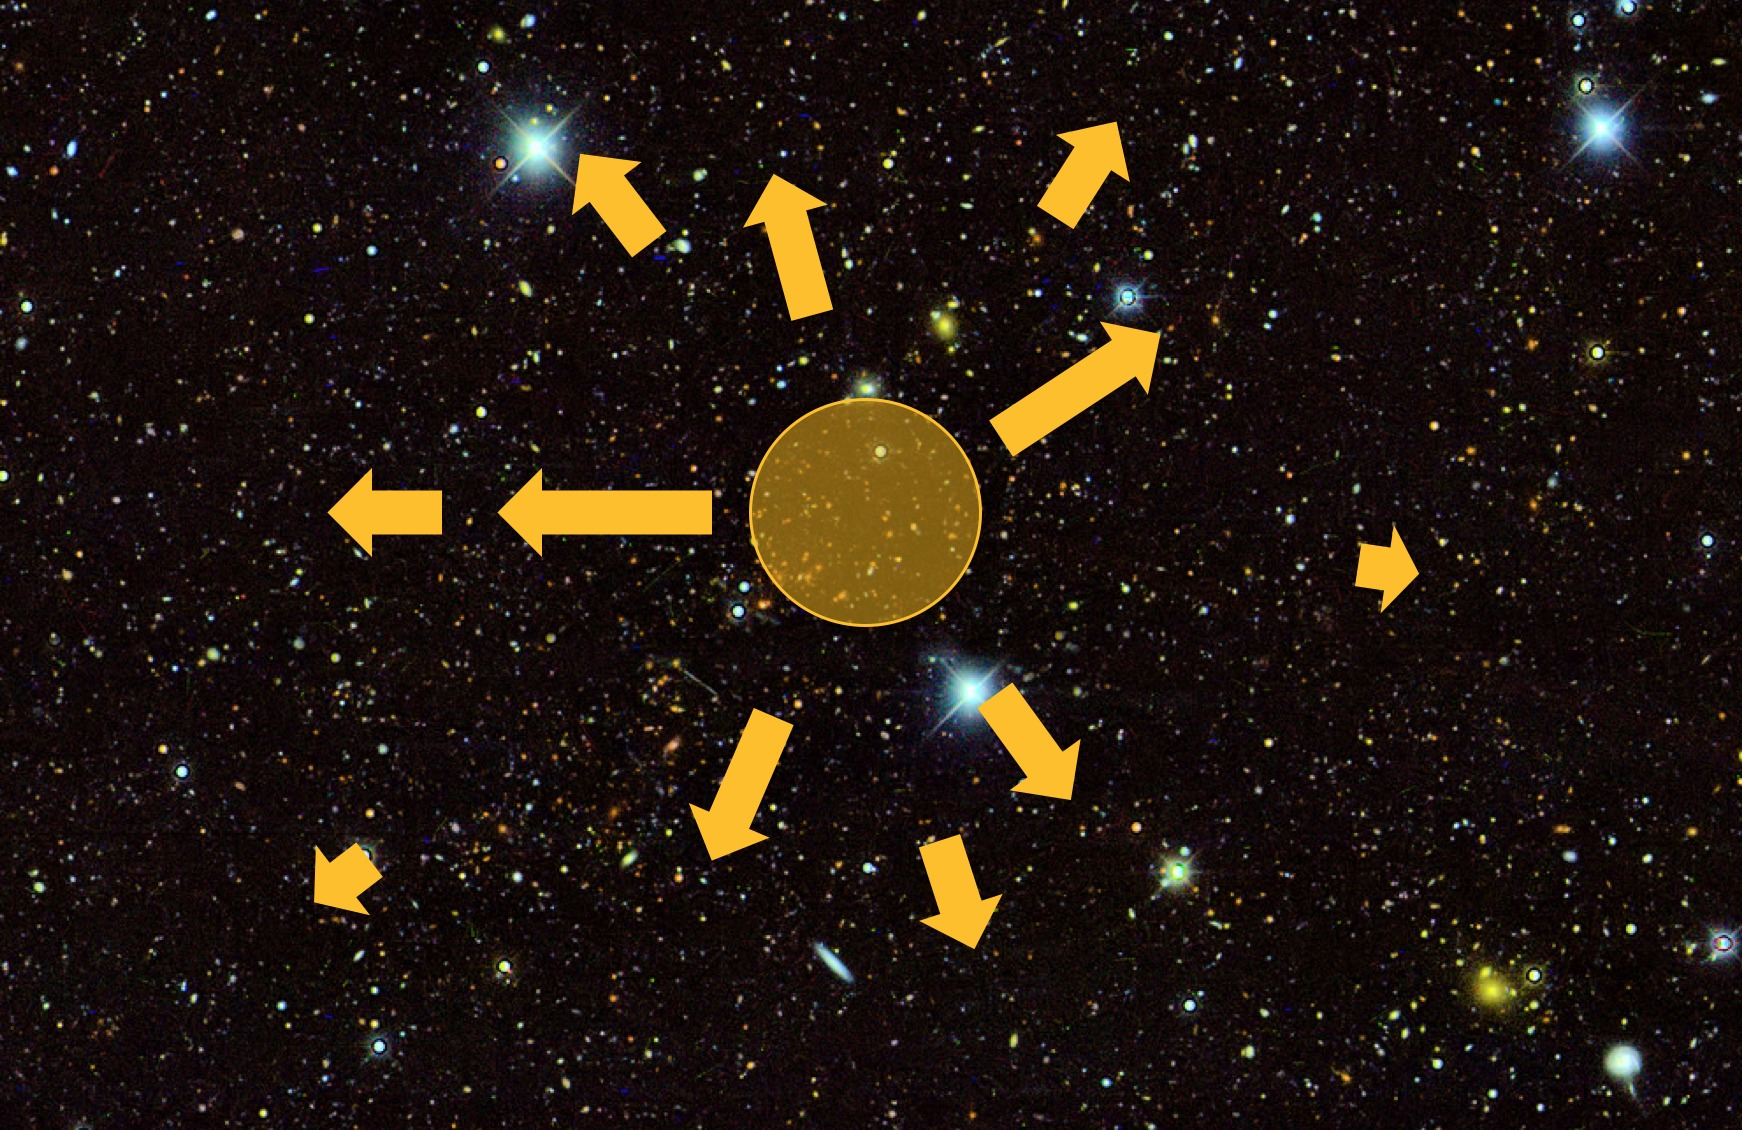
\includegraphics[scale=0.33]{figs/clusterfig.jpg}
  \end{center}
  \caption{
{\bf Cartoon of the impact of a foreground lens on
  background galaxies.} All galaxies appear further away from the
  cluster center, their observed positions shifting as
  indicated by the arrows. Galaxies closest to the center experience
  the largest shift in position (this 
lensing deflection is not shown to scale). The correlation function
of the background galaxies will also be distorted by these deflection
angles, and this is what we plan to measure.}
  \label{cluster}
\end{figure}

This is simplest to envision and to measure when measuring $w$ behind a massive object such as a galaxy cluster. 
Fig.~\ref{cluster} shows a schematic picture of this. For example, the positions of the two galaxies directly to the left of the cluster are deflected by different amounts (the one closest is deflected more than the one further away, so the observed distance between those two galaxies is {\it smaller} than it would be in the absence of lensing. The observed $w$ then is governed by the larger unlensed distance. Walking through this exercise for all pairs of galaxies in the picture make it clear that the observed $w$ will not depend on simply the observed angular distance between pairs of galaxies. Indeed, we argue that {\bf the 
most impactful implementation of the \atf\ of galaxies will be to measure the masses of galaxy clusters.}


%
%
%This assumption breaks down in the real universe where different lines
%of sight pass through over- or under-dense regions. The observed
%angular correlation therefore depends on the angular positions of the
%two galaxies: $w=w(\vec\theta_1 ,\vec\theta_2)\ne
%w(\vert\vec\theta_1-\vec\theta_2\vert)$. We propose to use this {\it
%  anisotropy of the correlation function} to learn about the structure
%between us and the background galaxies. We will first detect this
%behind the most massive objects, galaxy clusters, and then move to
%measure the anisotropy on the full sky, where it is induced by the
%various under- and over-dense regions that constitute the cosmic
%web. To be clear, the variety of non-gaussian effects that impact the
%distribution of galaxies on the sky do {\it not} break isotropy so
%cannot be confused with this effect.

\subsubsection{Context}

Galaxy clusters are the largest, most massive bound structures in the
universe and therefore are the key to a number of cosmological
puzzles. Chief among these is identifying the mechanism responsible
for the current epoch of cosmic acceleration. The community has moved
on from simply measuring the equation of state of a hypothetical dark
energy substance. There is now a concerted effort to test the
canonical $ \Lambda$CDM predictions both for the expansion history of
the universe and for the rate of the growth of structure. Galaxy
clusters offer the potential for testing both of these predictions:
the number of rare objects such as clusters at a given time is
exponentially sensitive to the RMS fluctuations in the density field,
so cluster abundance at multiple redshifts can be translated into measurements of the growth function. Similarly, the abundance is
sensitive to the volume of a given redshift slice, which depends on
the redshift-distance relation.

The one impediment to date of using clusters as a powerful tool is the
uncertainty in cluster masses. However, we are entering an exciting
epoch that promises to change this situation. Besides the large
surveys now online and coming online in the 2020's, five ways of
inferring cluster masses have emerged and using all of them together
leads to the hope that the systematic uncertainties in any one of them
will not induce a large bias. The techniques of interest are: cluster
richness, X-Ray luminosity, Sunyaev-Zel'dovich signal induced by hot
electrons in the intracluster gas, weak lensing by galaxies, and most
recently weak lensing by the cosmic microwave background 
(CMB)~\cite{Liu:2014pqa,Baxter:2014frs,2014MNRAS.439.1628Z,melchior2017,simet2017,Baxter:2017ixz}. This
proposal aims to add yet another tool that can measure galaxy cluster
masses. Dodelson has not only helped launch the field of CMB cluster lensing with \cite{Baxter:2014frs}, but also serves as Co-Chair of the
Dark Energy Survey Science Committee. He brings insight into the DES cluster cosmology analysis. The Year 1 analysis will be released by the time this proposal is read, and we are currently working on Year 3 data. From the estimates below, it is possible that \atf\ of galaxies will emerge as a powerful tool for cluster cosmology even for DES data. The situation is even more promising for next generation surveys, such as LSST.



%Of course, using the anisotropy in clustering
%statistics has been exploited already in studies of the cosmic
%microwave background.  The small scale structure of the CMB carries
%information about the lensing potential along the line of sight. This
%information has now been extracted by multiple CMB experiments,
%obtaining maps of the integrated gravitational potential and
%information about the masses of clusters. There are differences
%between the lensing-induced anisotropies proposed here and those
%produced by lensing of the CMB. First, the information in the CMB is
%currently limited by the resolution of the telescopes to be about
%$1'$, while galaxy surveys that measure galaxies do much better,
%resolving galaxies separated by several arcseconds. Second, the
%primary CMB is predominantly a Gaussian field, while the small scale
%galaxy distribution has evolved to be very non-gaussian\footnote{A
%  technical point: the impact of lensing produces an anisotropic field
%  in both the cases of the CMB and galaxy clustering. In the former
%  case, the anisotropic field is Gaussian, while in the latter it is
%  non-gaussian. In both cases, though, the effect is characterized by
%  $w\ne w(\vert\vec\theta_1-\vec\theta_2\vert)$.  The distinction between the Gaussian (CMB) and non-Gaussian (galaxies) manifestations
%  of lensing disappears when one considers the power spectra of the
%  lensing field: these are estimated via a 4-point function, which is
%  non-gaussian in both cases.}.
%
%The difference in scales suggests that the route into this new effect
%of the clustering anisotropy induced by lensing is by first detecting
%it when the lenses are discrete objects such as clusters. Upcoming
%surveys will find hundreds of galaxies -- and therefore tens of
%thousands of pairs of galaxies -- in the few square arcminute field
%behind a galaxy cluster. As we show below, this leads to an exciting
%opportunity to open up this new area of lensing. The fact that the
%signal scales with the number of pairs of galaxies and the fact that
%the shapes of these galaxies do not need to be measured reflect two
%advantages over the current weak lensing estimates of cluster
%masses. After detecting this effect behind clusters, we will turn to
%large scale mapping of the integrated gravitational potential. Here,
%the problem becomes similar to the CMB because the galaxy field on
%large scales is close to gaussian, so many of the tools developed in
%CMB lensing can be imported. Indeed, cross-correlating the maps
%produced by the CMB and those produced by galaxy fields will be a
%powerful way to reduce the systematic effects that afflict each
%separately.
%



\subsubsection{Estimates of detectability}

Let us provide a rough estimate of the detectability of
lensing-induced anisotropy in the galaxy distribution. Consider many
galaxies behind a massive galaxy cluster, with a known correlation
function $w(\theta)$. This assumption is important, but it is also
completely realistic because we will be able to measure the
correlation function over an entire survey so will have millions of
regions of roughly the size we are considering (ten square
arcminutes). When we average $w$ over all these regions, we will
obtain an excellent estimate of it on arcminute scales. The observed
correlation function will be distorted due to the presence of the
foreground lens, as in the cartoon in Fig.~\ref{cluster}. Each
galaxy's position will be shifted: \be \vec\theta^{\rm obs} =
\vec\theta + \vec{\delta\theta}(\vec\theta) \ee where $\vec\theta$ is
the undeflected positions, and the deflection angle $\vec
{\delta\theta}$ is a function of $\vec\theta$ that depends on the mass
distribution of the lens. In the simplest example of a point mass
lens, \be \vec{\delta\theta}(\vec\theta) =
\vec\theta\,\frac{\theta_E^2}{\theta^2} \ee where $\theta_E$ is the
Einstein radius of the lens, which could be as large as $1'$ for a
very massive cluster.






The unlensed positions are $\vec\theta^{\rm obs}-\vec{\delta\theta}$,
and the correlation function governing those unlensed positions is
$w(\theta)$. Therefore, the observed angular correlation function
between two positions $\vec\theta_ i$ and $\vec\theta_j$ is \be w^{\rm
  obs}(\vec\theta_i^{\rm obs},\vec\theta_j^{\rm obs}) = w(\vert
\vec\theta _i^{\rm obs} - \vec{\delta\theta}(\vec\theta_i) -
\vec\theta_j^{\rm obs} + \vec {\delta\theta}(\vec\theta_j)\vert).  \ee
For the purposes of estimating the magnitude of this effect, we now
make the approximation that the deflections are small, so the
argument of $w$ on the right -hand side can be Taylor expanded. Note
that this approximation is not essential, as in the case of CMB
cluster lensing~\cite{Baxter:2014frs} we avoided it by using a likelihood approach, but
this will be the first step in our program. Taylor expanding and dropping the $^{\rm obs}$ superscript on the angles leads to \bea
w^{\rm obs}(\vec\theta_i,\vec\theta_j) &=& w(\theta_{ij}) +
w'(\theta_{ij})\left[ \vec{\delta\theta}(\vec\theta_i) -
\vec{\delta\theta}(\vec\theta_j) \right]\cdot
\frac{\vec\theta_i-\vec\theta_j}{\vert
  \vec\theta_i-\vec\theta_j\vert}\vs &\equiv &w(\theta_{ij}) +
w'(\theta_{ij}) f_{ij} \eql{taylor} \eea where here $\theta_{ij}\equiv
\vert\vec\theta_i-\vec\theta_j\vert$; $w'\equiv d w/d\theta$, which
can be measured extremely accurately from all other patches in the
survey; and the second line condenses the additional terms to save
space.


The second term in \ec{taylor} is the effect we are after, the signal,
as it contains the information about the deflection angles that
depend on the mass of the lens. To estimate the signal to noise, we
imagine pixelizing the region around the lens and forming an
estimator for the angular correlation function for every pixel pair:
\be \hat w(\vec\theta_i,\vec\theta_j) = \delta_i\delta_j \ee where
$\delta_i\equiv (n_i-\bar n)/\bar n$. Here $n_i$ is the number of
galaxie s in pixel $i$ and for simplicity it is assumed that the
expected number of gal axies in each pixel is equal to $n$ (i.e., it
is assumed that the mask is trivi al). This estimator for $w$ is the
Landy and Szalay estimator~\cite{1993ApJ...412...64L}, with an expectation value equal to
\ec{taylor}.  As a first estimate, we neglect cosmic variance, so
that the error on the estimator is simply Poisson noise: \be {\rm
  Var}(\hat w) = \frac{1}{\bar n^2} .\ee The signal to noise squared
then is \be \left(\frac{S}{N}\right)^2 = \sum_{ij}
\frac{\left(w'(\theta_{ij})f_{ij}\right )^2}{1/\bar n^2} \ee
Fig.~\rf{fthij} shows $f_{ij}/\theta_{ij}$ ( which multiplies
$dw/d\ln(\theta)$ in the sum for all pairs of pixels. Of course pixels
closest to the center of the cluster contribute the most to the signal
to noise.

\Sfig{figs/fthij}{Contribution to the signal to noise on the
  lensing-induced anisotropy from pairs of pixels as a function of
  the distance of the first pixel to the center. Here the cluster is
  taken to have an Einstein radius of $0.5'$, and a square region of
  $50$ square arcmin is used in the sum, with 169 pixels covering the
  area.}

In the example depicted in the figure, the total signal to noise is
equal to \be \frac{S}{N} = 0.02 \frac{\bar n}{{\rm gal}/(1')^2}
\,\frac{dw/d\ln(\theta)}{10^ {-2}}.  .\ee Even for the Dark Energy
Survey, which can capture ten galaxies per square arcminute (recall that
shapes are not needed), this estimate for the signal to noise for a single cluster is
0.2. Therefore, stacking 1000 clusters will give a 6-sigma
detection. And upcoming surveys with the capability to go much deeper
will do considerably better, perhaps even detecting the effect on a
single massive cluster.

Of course this estimate needs to be fleshed out and tested on simulations; 
indeed, this is the main aim of a large part of the proposal (\S\ref{sec:sim}).






